\chapter{الجزيئات العضوية: الهياكل والأسماء}\label{ch:g11:organic-skeletons}

تحوي القداحة التي تُرمى بعد الاستعمال البيوتانَ، سائلًا تحت الضغط؛ وعبوة موقد
التخييم التي تُحمل إلى جبل مكسو بالثلج تحوي البروبان، أو مزيجًا غنيًا به. وكلاهما
لا يتكوّن إلا من \omterm{def:g7:atoms-and-molecules:atom}{ذرات} الكربون والهيدروجين، وكلاهما ينتمي إلى عائلة هائلة: \omterm{def:g7:atoms-and-molecules:molecule}{الجزيئات}
المبنية على هيكل من \omterm{def:g7:atoms-and-molecules:atom}{ذرات} الكربون. وهي تُعدّ بالملايين. وللحديث عنها يحتاج
الكيميائيون إلى طرائق لرسمها بسرعة وتسميتها دون لبس.

\begin{recall}
يكوّن الكربون أربع روابط تساهمية والهيدروجين رابطة واحدة؛ وحول \omterm{def:g7:atoms-and-molecules:atom}{ذرة} كربون لها
أربع روابط أحادية تتجه الروابط إلى رؤوس رباعي أوجه،
بزاوية نحو \ang{109.5} (\cref{ch:g10:lewis-and-shape}).
\end{recall}

\begin{omfigure}
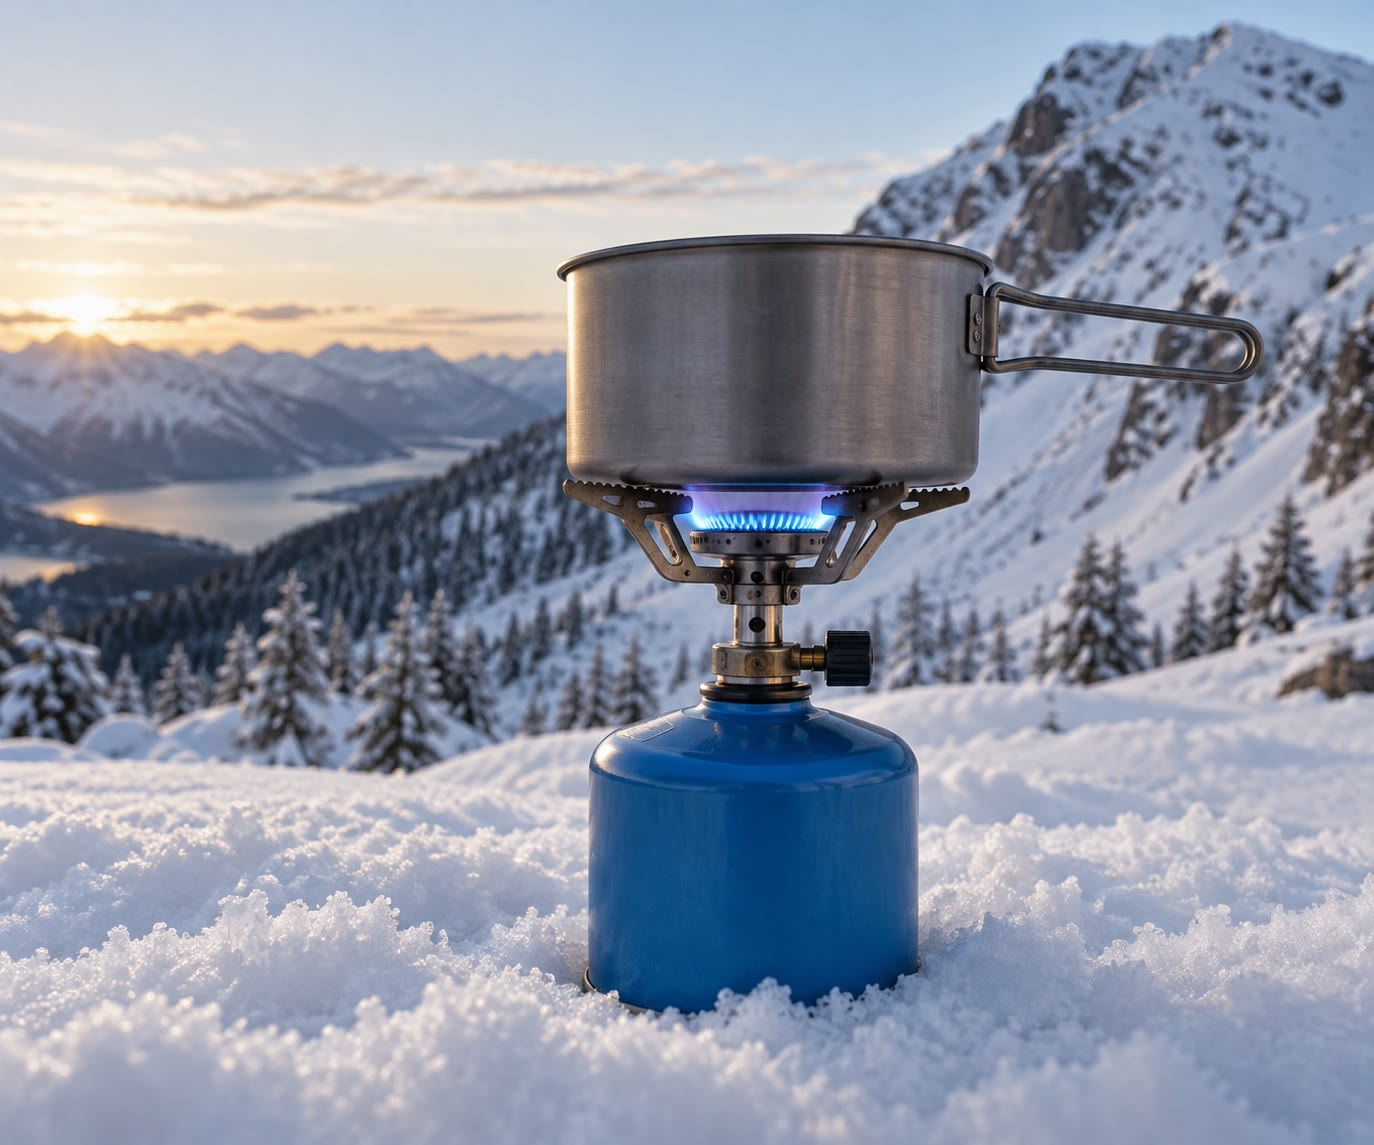
\includegraphics[width=0.48\linewidth]{images/book1/ai/g11-camping-cartridge.jpg}

{\small موقد تخييم في الثلج، يحرق غازًا مكوّنًا من الكربون
والهيدروجين.}
\end{omfigure}

\section{صيغ الجزيئات العضوية}

\begin{definition}[المركب العضوي]\label{def:g11:organic-skeletons:organic}
\emph{المركب العضوي}\index{مركب عضوي} مركب جزيئاته مبنية على هيكل من \omterm{def:g7:atoms-and-molecules:atom}{ذرات}
كربون مرتبط بعضها ببعض وبذرات هيدروجين، وقد تكون معها \omterm{def:g7:atoms-and-molecules:atom}{ذرات} أخرى مثل الأكسجين
والنيتروجين. (ويُستثنى تقليديًا ثنائي أكسيد الكربون وأول أكسيد الكربون
والكربونات.)
\end{definition}

\begin{definition}[أربعة أنواع من الصيغ]\label{def:g11:organic-skeletons:formulas}
يمكن كتابة \omterm{def:g7:atoms-and-molecules:molecule}{الجزيء} بأربع طرائق:
\begin{itemize}
  \item \emph{صيغته الجزيئية}\index{صيغة جزيئية} لا تعطي إلا عدد
        \omterm{def:g7:atoms-and-molecules:atom}{الذرات} من كل عنصر، مثل \ce{C4H10}؛
  \item \emph{صيغته البنيوية}\index{صيغة بنيوية} تُظهر
        كل \omterm{def:g7:atoms-and-molecules:atom}{ذرة} وكل رابطة؛
  \item \emph{صيغته نصف البنيوية}\index{صيغة نصف بنيوية}
        تُظهر الروابط بين \omterm{def:g7:atoms-and-molecules:atom}{ذرات} الكربون وتجمع \omterm{def:g7:atoms-and-molecules:atom}{ذرات} الهيدروجين
        مع كربونها، مثل \ce{CH3-CH2-CH2-CH3}؛
  \item \emph{صيغته الهيكلية}\index{صيغة هيكلية} لا ترسم إلا
        روابط الهيكل الكربوني خطًا متعرجًا: كل طرف وكل زاوية \omterm{def:g7:atoms-and-molecules:atom}{ذرة} كربون،
        \omterm{def:g7:atoms-and-molecules:atom}{وذرات} الهيدروجين على الكربون لا تُرسم، وكل \omterm{def:g7:atoms-and-molecules:atom}{ذرة} أخرى (مع \omterm{def:g7:atoms-and-molecules:atom}{ذرات}
        الهيدروجين المرتبطة بها) تُكتب.
\end{itemize}
\end{definition}

\begin{omfigure}
\setchemfig{atom sep=1.45em}
\renewcommand{\arraystretch}{1.6}
\small
\begin{tabular}{@{}l@{\quad}c@{\quad}c@{}}
 & البيوتان & 2-ميثيل بروبان \\
الجزيئية & \ce{C4H10} & \ce{C4H10} \\[4pt]
البنيوية &
\chemfig{H-C(-[2]H)(-[6]H)-C(-[2]H)(-[6]H)-C(-[2]H)(-[6]H)-C(-[2]H)(-[6]H)-H} &
\chemfig{H-C(-[2]H)(-[6]H)-C(-[6]H)(-[2,1.5]C(-[1]H)(-[3]H)(-[2]H))-C(-[2]H)(-[6]H)-H} \\[10pt]
نصف البنيوية & \ce{CH3-CH2-CH2-CH3} &
\chemfig{CH_3-CH(-[6]CH_3)-CH_3} \\[14pt]
الهيكلية & \chemfig{-[:30]-[:-30]-[:30]} & \chemfig{-[:30](-[:90])-[:-30]} \\
\end{tabular}

{\small الصيغ الأربع للبيوتان و2-ميثيل بروبان. في الصيغ الهيكلية كل طرف وكل
زاوية من الخطوط \omterm{def:g7:atoms-and-molecules:atom}{ذرة} كربون: أربع في كل
منهما.}
\end{omfigure}


\begin{example}[قراءة صيغة هيكلية]\label{ex:g11:organic-skeletons:reading}
في \omterm{def:g11:organic-skeletons:formulas}{الصيغة الهيكلية} للبيوتان للخط المتعرج طرفان وزاويتان: أي أربع \omterm{def:g7:atoms-and-molecules:atom}{ذرات} كربون.
ولكل كربون طرفي رابطة واحدة مرسومة، فهو يحمل ثلاث \omterm{def:g7:atoms-and-molecules:atom}{ذرات} هيدروجين (\ce{CH3})؛
ولكل زاوية رابطتان مرسومتان، فهي تحمل اثنتين (\ce{CH2}). ولكل كربون أربع
روابط في المجموع، وهذا يعيد إلينا \ce{C4H10}.
\end{example}

\section{السلاسل الكربونية}

قد يكون الهيكل الكربوني \omterm{def:g7:atoms-and-molecules:molecule}{لجزيء} سلسلة \emph{خطية}، كل كربون فيها مرتبط بذرتي
كربون على الأكثر، كما في البيوتان؛ أو سلسلة \emph{متفرعة}، فيها كربون واحد على
الأقل مرتبط بثلاث \omterm{def:g7:atoms-and-molecules:atom}{ذرات} كربون أو أربع، كما في 2-ميثيل بروبان؛ أو \emph{حلقة}،
كما في الهكسان الحلقي، \ce{C6H12}، \omterm{def:g11:organic-skeletons:formulas}{وصيغته الهيكلية} سداسي. ويُستعمل الخط المتعرج
للسلاسل لأن الروابط الحقيقية حول كل كربون تصنع زوايا نحو \ang{109.5}، لا
\ang{180}: فالسلسلة «الخطية» هي في الحقيقة خط متعرج في الفضاء.

\begin{omfigure}
\setchemfig{atom sep=1.9em}
\begin{tabular}{ccc}
\chemfig{-[:30]-[:-30]-[:30]-[:-30]-[:30]} &
\chemfig{-[:30](-[:90])-[:-30]-[:30](-[:90])-[:-30]} &
\chemfig{*6(------)} \\[4pt]
\small خطية: الهكسان & \small متفرعة: 2,4-ثنائي ميثيل بنتان &
\small حلقية: الهكسان الحلقي \\
\small \ce{C6H14} & \small \ce{C7H16} & \small \ce{C6H12}
\end{tabular}

{\small ثلاثة هياكل كربونية، بالصيغ الهيكلية.}
\end{omfigure}

\section{الألكانات وأسماؤها}

\begin{definition}[الألكان، ومجموعة الألكيل]\label{def:g11:organic-skeletons:alkane}
\emph{الألكان}\index{ألكان} مركب من الكربون والهيدروجين هيكله سلسلة
(خطية أو متفرعة، لا حلقة) ليس فيها إلا روابط أحادية؛ \omterm{def:g11:organic-skeletons:formulas}{وصيغته الجزيئية}
\ce{C_{n}H_{2n+2}}. و\emph{مجموعة الألكيل}\index{مجموعة ألكيل}
هي ما يبقى من الألكان حين تُنزع منه \omterm{def:g7:atoms-and-molecules:atom}{ذرة} هيدروجين واحدة، حتى يمكن ربطه
بسلسلة: الميثيل \ce{-CH3}، والإيثيل \ce{-CH2-CH3}.
\end{definition}

\begin{omfigure}
\begin{tabular}{rlcrlc}
\hline
$n$ & الاسم & الصيغة & $n$ & الاسم & الصيغة \\
\hline
1 & الميثان & \ce{CH4}    & 6  & الهكسان & \ce{C6H14} \\
2 & الإيثان  & \ce{C2H6}   & 7  & الهبتان & \ce{C7H16} \\
3 & البروبان & \ce{C3H8}   & 8  & الأوكتان & \ce{C8H18} \\
4 & البيوتان  & \ce{C4H10}  & 9  & النونان & \ce{C9H20} \\
5 & البنتان & \ce{C5H12}  & 10 & الديكان & \ce{C10H22} \\
\hline
\end{tabular}\par\medskip

{\small الألكانات الخطية العشرة الأولى. اسم سلسلة من $n$ \omterm{def:g7:atoms-and-molecules:atom}{ذرة} كربون جذر ثابت يتبعه
المقطع \emph{ان}؛ \omterm{def:g11:organic-skeletons:alkane}{ومجموعة الألكيل} تستبدل بالمقطع \emph{ان} المقطع
\emph{يل} (ميثيل، إيثيل، بروبيل\dots).}
\end{omfigure}

\begin{method}[تسمية الألكان]\label{met:g11:organic-skeletons:naming}
\begin{enumerate}
  \item جد أطول سلسلة من \omterm{def:g7:atoms-and-molecules:atom}{ذرات} الكربون: فهي تعطي اسم الجذر
        (بنتان، هكسان\dots).
  \item \omterm{def:g7:atoms-and-molecules:atom}{الذرات} التي ليست فيها تكوّن مجموعات ألكيل مرتبطة بها، هي
        المستبدِلات.
  \item رقّم السلسلة الرئيسية من الطرف الذي يعطي المستبدِلات
        أصغر الأرقام.
  \item اكتب كل مستبدِل مع رقمه (موقعه على
        السلسلة)، بالترتيب الأبجدي لأسمائها الدولية، قبل الجذر؛ والمجموعات المتكررة
        تأخذ البوادئ ثنائي، وثلاثي، ورباعي، مع رقم لكل منها.
        وتُفصل الأرقام بفواصل، والأرقام عن الكلمات بشرطات.
\end{enumerate}
\end{method}

\begin{omfigure}
\begin{tikzpicture}[font=\small, x=0.9cm, y=0.9cm]
  % main chain of 5, zigzag; methyls on C2 and C3
  \coordinate (a1) at (0,0); \coordinate (a2) at (0.87,0.5);
  \coordinate (a3) at (1.73,0); \coordinate (a4) at (2.6,0.5);
  \coordinate (a5) at (3.46,0);
  \coordinate (m2) at (0.87,1.5); \coordinate (m3) at (1.73,-1);
  \draw[line width=1pt] (a1) -- (a2) -- (a3) -- (a4) -- (a5);
  \draw[line width=1pt] (a2) -- (m2); \draw[line width=1pt] (a3) -- (m3);
  \foreach \k in {1,2,3,4,5}
    \node[omDef, font=\footnotesize\bfseries, fill=white, inner sep=1pt]
      at ($(a\k)+(0,-0.32)$) {\k};
  \draw[omProp, thick] (m2) circle (0.28);
  \draw[omProp, thick] (m3) circle (0.28);
  \node[omProp, anchor=west] at ($(m2)+(0.35,0)$) {ميثيل على C2};
  \node[omProp, anchor=west] at ($(m3)+(0.35,0)$) {ميثيل على C3};
  \node[anchor=west, align=left] at (5,0.3) {\foreignlanguage{arabic}{أطول سلسلة: \babelsublr{5} ذرات كربون،
    \emph{بنتان}}\\ \foreignlanguage{arabic}{ترقيم من اليسار: \babelsublr{2} و\babelsublr{3}}\\ (\foreignlanguage{arabic}{من اليمين: \babelsublr{3}
    و\babelsublr{4}، أكبر})\\ \foreignlanguage{arabic}{الاسم: \textbf{\babelsublr{2,3}-ثنائي ميثيل بنتان}}};
\end{tikzpicture}

{\small تسمية \omterm{def:g11:organic-skeletons:alkane}{ألكان} متفرع: السلسلة الرئيسية (مرقّمة)، والمستبدِلات (داخل
دوائر)، والاسم.}
\end{omfigure}

\begin{method}[من الاسم إلى الصيغة الهيكلية]\label{met:g11:organic-skeletons:drawing}
\begin{enumerate}
  \item ارسم السلسلة الرئيسية التي يعطيها الجذر، خطًا متعرجًا، ورقّم
        \omterm{def:g7:atoms-and-molecules:atom}{ذرات} كربونها.
  \item اربط كل مستبدِل في الموقع الذي يعطيه رقمه.
  \item تحقق: عُدّ \omterm{def:g7:atoms-and-molecules:atom}{ذرات} الكربون، وتأكد من أنه لا توجد \omterm{def:g7:atoms-and-molecules:atom}{ذرة} كربون لها أكثر من
        أربع روابط.
\end{enumerate}
\end{method}

\section{المتماكبات}

\begin{definition}[المتماكبات، والمتماكبات البنيوية]\label{def:g11:organic-skeletons:isomer}
\emph{المتماكبات}\index{متماكبات} مركبات مختلفة لها \omterm{def:g11:organic-skeletons:formulas}{الصيغة الجزيئية}
نفسها. و\emph{المتماكبات البنيوية}\index{متماكبات بنيوية}
متماكبات ترتبط ذراتها بترتيب مختلف، مثل أن
يكون لها هيكل كربوني مختلف.
\end{definition}

\begin{proposition}[للمتماكبات خصائص مختلفة]\label{prop:g11:organic-skeletons:properties}
% ledger: bp:C4H10, bp:isobutane, bp:C5H12, bp:isopentane, bp:neopentane
\omterm{def:g11:organic-skeletons:isomer}{المتماكبات البنيوية} مواد مختلفة، لها خصائص مختلفة. ومن بين \omterm{def:g11:organic-skeletons:isomer}{متماكبات} \omterm{def:g11:organic-skeletons:alkane}{الألكان} ذات
الصيغة الواحدة، الأكثر تفرعًا يغلي عند درجة أدنى: فالبيوتان يغلي قرب
\qty{0}{\celsius} و2-ميثيل بروبان عند \qty{-11.7}{\celsius}؛ والبنتان عند
\qty{36.1}{\celsius}، و2-ميثيل بيوتان عند \qty{27.8}{\celsius}
و2,2-ثنائي ميثيل بروبان عند \qty{9.5}{\celsius}.
\end{proposition}

\begin{proof}
القيم مقيسة. \omterm{def:g7:atoms-and-molecules:molecule}{والجزيئات} المتفرعة أكثر تراصًّا، وسطحها الملامس لجيرانها أصغر: فتآثرات
فان دير فالس بينها أضعف
(\cref{ch:g11:polarity-and-cohesion}).
\end{proof}

\begin{omfigure}
\setchemfig{atom sep=2em}
\begin{tabular}{ccc}
\chemfig{-[:30]-[:-30]-[:30]-[:-30]} &
\chemfig{-[:30](-[:90])-[:-30]-[:30]} &
\chemfig{-[:0](-[:90])(-[:-90])-[:0]} \\[24pt]
\small البنتان & \small 2-ميثيل بيوتان & \small 2,2-ثنائي ميثيل بروبان \\
\small \qty{36.1}{\celsius} & \small \qty{27.8}{\celsius} &
\small \qty{9.5}{\celsius}
\end{tabular}
\medskip

{\small \omterm{def:g11:organic-skeletons:isomer}{المتماكبات} الثلاثة للصيغة \ce{C5H12} ودرجات غليانها: كلما زاد التفرع
انخفضت.}
\end{omfigure}

\section{الألكانات من النفط الخام}

النفط الخام \omterm{def:g6:pure-substances-and-mixtures:mixture}{خليط} من آلاف المركبات، معظمها ألكانات فيها من \omterm{def:g7:atoms-and-molecules:atom}{ذرة} كربون واحدة إلى أكثر
من 40 \omterm{def:g7:atoms-and-molecules:atom}{ذرة}. وفي المصفاة يُسخَّن وتصعد أبخرته في برج طويل، يبرد أكثر فأكثر نحو
الأعلى: فيتكثف كل جزء عند الارتفاع الذي توافق فيه درجة الحرارة مجال غليانه.
فتخرج الغازات (من الميثان إلى البيوتان) من الأعلى، ثم البنزين، والكيروسين،
والديزل؛ وتبقى الزيوت الثقيلة والقار في الأسفل. وهذا \omterm{def:g10:chemical-species:distillation}{التقطير} التجزيئي يفصل بحسب
درجة الغليان، التي تزداد في الألكانات مع طول السلسلة.

\begin{omfigure}
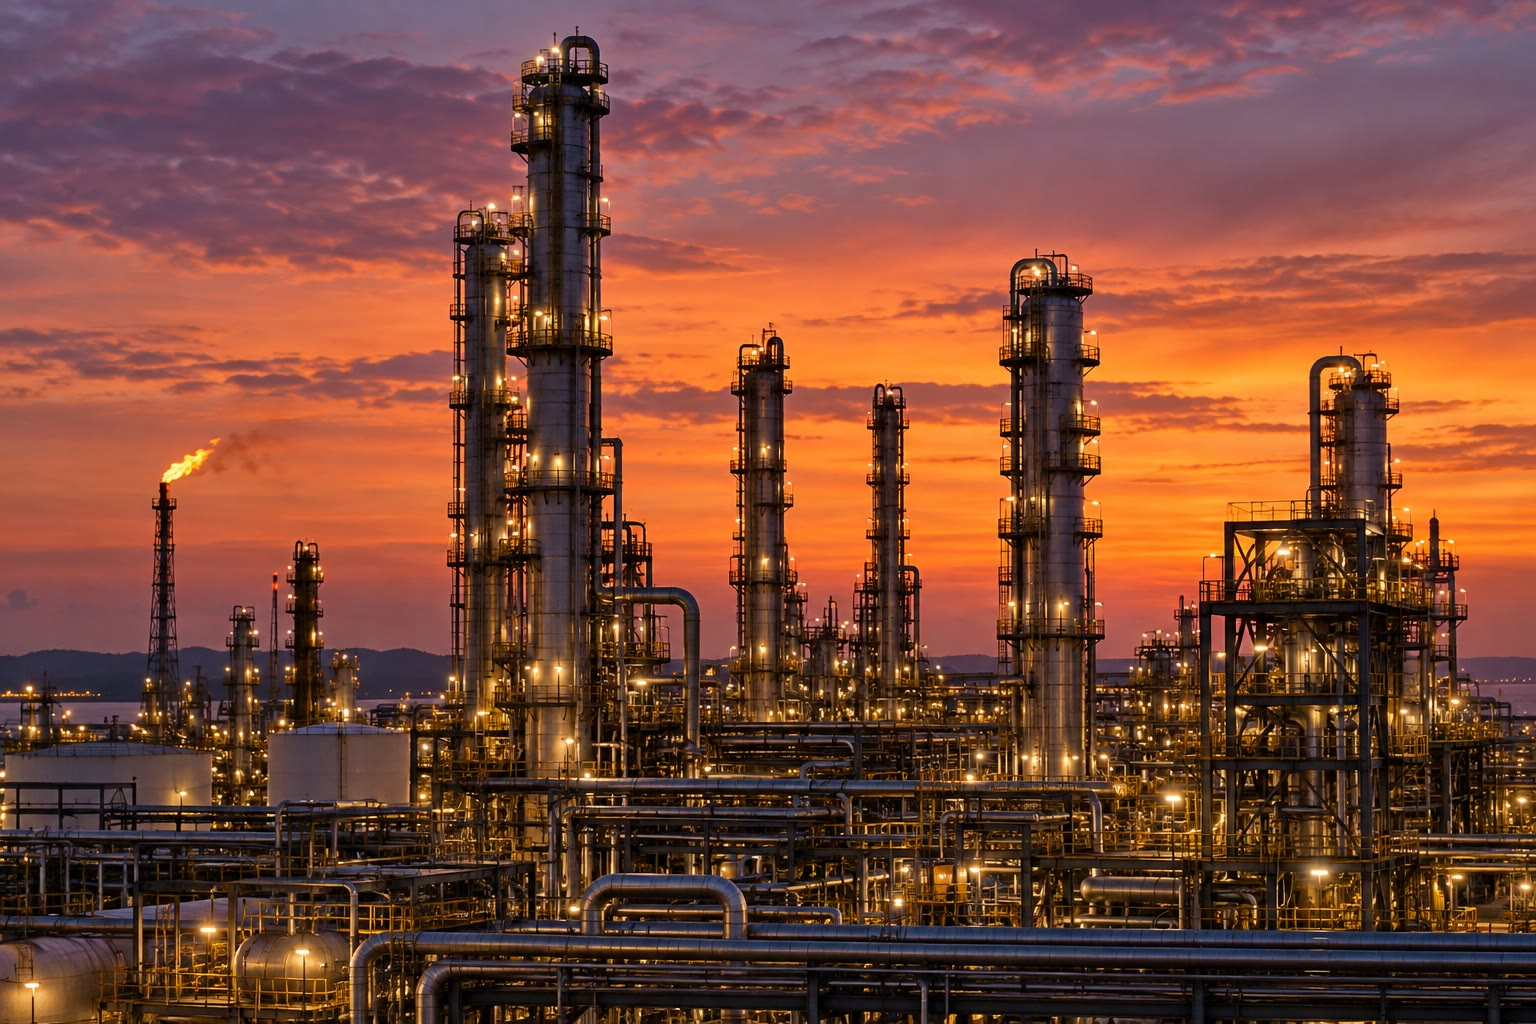
\includegraphics[width=0.52\linewidth]{images/book1/ai/g11-refinery-dusk.jpg}

{\small أبراج \omterm{def:g10:chemical-species:distillation}{تقطير} في مصفاة عند الغسق.}
\end{omfigure}

\begin{safety}{\ghs[0.66cm]{GHS02}\ghs[0.66cm]{GHS04}\ghs[0.66cm]{GHS07}\ghs[0.66cm]{GHS08}\ghs[0.66cm]{GHS09}}
% ledger: ghs:butane, ghs:pentane
البيوتان غاز شديد القابلية للاشتعال، يُخزَّن تحت الضغط. والبنتان سائل شديد القابلية
للاشتعال؛ وبخاره يسبب النعاس، وقد يؤذي الرئتين إذا ابتُلع، وهو سام للأحياء
المائية. لا لهب قرب الألكانات الخفيفة؛ والعمل تحت ساحبة
الغازات.
\end{safety}

\section{تمارين}


\begin{exercise}[$\star$]\label{exo:g11:organic-skeletons:1}
أعطِ الصيغ الجزيئية للجزيئين المرسومين هنا، وقل هل هما
متماكبان:
\setchemfig{atom sep=1.6em}
\chemfig{-[:30]-[:-30]-[:30]-[:-30]-[:30]} \quad و\quad
\chemfig{-[:30](-[:90])-[:-30]-[:30]-[:-30]}.
\end{exercise}

\begin{exercise}[$\star$]\label{exo:g11:organic-skeletons:2}
سمِّ: \ce{CH3-CH2-CH3}؛ \ce{CH3-CH2-CH2-CH2-CH2-CH3}؛
\chemfig{CH_3-CH(-[2]CH_3)-CH_2-CH_3}.
\end{exercise}

\begin{exercise}[$\star$]\label{exo:g11:organic-skeletons:3}
اكتب الصيغتين نصف البنيويتين للبروبان و2-ميثيل بروبان،
\omterm{def:g11:organic-skeletons:formulas}{والصيغة البنيوية} للإيثان.
\end{exercise}

\begin{exercise}[$\star$]\label{exo:g11:organic-skeletons:4}
عُدّ \omterm{def:g7:atoms-and-molecules:atom}{ذرات} الكربون والهيدروجين في كل \omterm{def:g7:atoms-and-molecules:molecule}{جزيء}:
\setchemfig{atom sep=1.6em}
\chemfig{-[:30]-[:-30](-[:-90])-[:30]-[:-30]} \quad و\quad
\chemfig{*6(------)}.
\end{exercise}

\begin{exercise}[$\star$]\label{exo:g11:organic-skeletons:5}
أعطِ \omterm{def:g11:organic-skeletons:formulas}{الصيغة الجزيئية} \omterm{def:g11:organic-skeletons:alkane}{للألكان} الذي فيه 8 \omterm{def:g7:atoms-and-molecules:atom}{ذرات} كربون، وعدد \omterm{def:g7:atoms-and-molecules:atom}{ذرات} الكربون في
\omterm{def:g11:organic-skeletons:alkane}{الألكان} الذي فيه 20 \omterm{def:g7:atoms-and-molecules:atom}{ذرة} هيدروجين.
\end{exercise}

\begin{exercise}[$\star\star$]\label{exo:g11:organic-skeletons:6}
ارسم الصيغ الهيكلية للمركبات 3-ميثيل هكسان و2,2-ثنائي ميثيل بيوتان
و3-إيثيل بنتان، وأعطِ صيغها الجزيئية.
\end{exercise}

\begin{exercise}[$\star\star$]\label{exo:g11:organic-skeletons:7}
ارسم \omterm{def:g11:organic-skeletons:isomer}{المتماكبات} الثلاثة للصيغة \ce{C5H12} وسمّها.
\end{exercise}

\begin{exercise}[$\star\star$]\label{exo:g11:organic-skeletons:8}
هذه الأسماء خاطئة. ارسم كل \omterm{def:g7:atoms-and-molecules:molecule}{جزيء} وأعطِ اسمه الصحيح:
2-إيثيل بيوتان؛ 4-ميثيل بنتان؛ 1-ميثيل بيوتان.
\end{exercise}

\begin{exercise}[$\star\star$]\label{exo:g11:organic-skeletons:9}
مستعينًا بشكل \omterm{def:g11:organic-skeletons:isomer}{متماكبات} \ce{C5H12}، رتّبها بحسب درجة
الغليان وفسّر الترتيب.
\end{exercise}

\begin{exercise}[$\star\star$]\label{exo:g11:organic-skeletons:10}
الهكسان الحلقي \ce{C6H12} والهكسان \ce{C6H14}. فسّر ذرتي الهيدروجين
الناقصتين. وهل المركبان متماكبان؟ وهل الهكسان الحلقي
\omterm{def:g11:organic-skeletons:alkane}{ألكان}؟
\end{exercise}

\begin{exercise}[$\star\star$]\label{exo:g11:organic-skeletons:11}
من بين البروبان والبيوتان و2-ميثيل بروبان والبيوتان الحلقي (\ce{C4H8}، حلقة
من أربع \omterm{def:g7:atoms-and-molecules:atom}{ذرات} كربون)، أيها \omterm{def:g11:organic-skeletons:isomer}{متماكبات} بعضها لبعض؟
\end{exercise}

\begin{exercise}[$\star\star\star$]\label{exo:g11:organic-skeletons:12}
ارسم \omterm{def:g11:organic-skeletons:isomer}{المتماكبات} الخمسة للصيغة \ce{C6H14} وسمّها.
\end{exercise}

\begin{exercise}[$\star\star\star$]\label{exo:g11:organic-skeletons:13}
تصوّر \omterm{def:g11:organic-skeletons:alkane}{الألكان} الخطي خطًا متعرجًا طويلًا \omterm{def:g11:organic-skeletons:alkane}{والألكان} الكثير التفرع كرة. مستعينًا بهذه
الصورة، اشرح لماذا يخفض التفرع درجة غليان
\omterm{def:g11:organic-skeletons:isomer}{المتماكبات}.
\end{exercise}

\begin{exercise}[$\star\star\star$]\label{exo:g11:organic-skeletons:14}
سمِّ \omterm{def:g11:organic-skeletons:alkane}{الألكان}
\begin{center}
\chemfig{CH_3-CH(-[2]CH_3)-CH_2-C(-[2]CH_3)(-[6]CH_3)-CH_2-CH_3}
\end{center}
\end{exercise}

\begin{exercise}[$\star\star\star$]\label{exo:g11:organic-skeletons:15}
المركب المرجعي للبنزين، «الأيزوأوكتان»، هو
2,2,4-ثلاثي ميثيل بنتان. ارسم \omterm{def:g11:organic-skeletons:formulas}{صيغته الهيكلية}، وتحقق من أنه
متماكب للأوكتان، واكتب \omterm{def:g11:organic-skeletons:formulas}{صيغته نصف البنيوية}.
\end{exercise}

\section{مسألة: غاز القداحة}

\begin{problem}[{مسألة نهاية الأسبوع --- كم ألكانًا مختلفًا له
الصيغة \ce{C7H16}؟}]
\label{pb:g11:organic-skeletons:1}
% ledger: bp:C3H8, bp:C4H10, bp:isobutane
تحوي القداحة البيوتان؛ وتحوي عبوة التخييم الشتوية مزيجًا أغنى
بالبروبان أو بالمركب 2-ميثيل بروبان. يغلي البيوتان عند نحو
\qty{0}{\celsius}، و2-ميثيل بروبان عند \qty{-11.7}{\celsius}، والبروبان
عند \qty{-42}{\celsius}.

\medskip
\noindent\textbf{الجزء الأول --- غازان بصيغة واحدة.}
\begin{enumerate}
  \item أعطِ \omterm{def:g11:organic-skeletons:formulas}{الصيغة الجزيئية} للبيوتان، وتحقق من أنها توافق
        الصيغة العامة للألكانات.
  \item ارسم \omterm{def:g11:organic-skeletons:formulas}{صيغته البنيوية}.
  \item اكتب صيغتيه نصف البنيوية والهيكلية.
  \item ارسم 2-ميثيل بروبان بالطرائق الثلاث نفسها. لماذا له
        \omterm{def:g11:organic-skeletons:formulas}{الصيغة الجزيئية} نفسها؟
  \item هل البيوتان و2-ميثيل بروبان متماكبان؟ ومن أي نوع؟
\end{enumerate}

\medskip
\noindent\textbf{الجزء الثاني --- في البرد.}
\begin{enumerate}[resume]
  \item أي الغازات الثلاثة غازات عند \qty{20}{\celsius} والضغط
        العادي؟
  \item تُستعمل قداحة مفتوحة في الخارج عند \qty{-5}{\celsius}. لماذا
        تعطي لهبًا ضعيفًا؟
  \item لماذا تكون العبوات الشتوية غنية بالبروبان أو بالمركب 2-ميثيل بروبان؟
  \item اشرح لماذا يغلي 2-ميثيل بروبان عند درجة أدنى من البيوتان.
  \item لماذا ليس للبروبان متماكب؟
\end{enumerate}

\medskip
\noindent\textbf{الجزء الثالث --- التسمية والعدّ.}
\begin{enumerate}[resume]
  \item سمِّ \chemfig{CH_3-CH(-[2]CH_3)-CH_2-CH_3}.
  \item لماذا يكون الاسم «3-ميثيل بيوتان» خاطئًا \omterm{def:g7:atoms-and-molecules:molecule}{للجزيء} نفسه؟
  \item كم متماكبًا ألكانيًا للصيغ \ce{C4H10}،
        و\ce{C5H12}، و\ce{C6H14}؟
\end{enumerate}

\medskip
\noindent\textbf{الجزء الرابع --- \omterm{def:g11:organic-skeletons:isomer}{متماكبات} \ce{C7H16}.}
\begin{enumerate}[resume]
  \item ارسم المتماكب الخطي وسمّه.
  \item ارسم وسمِّ \omterm{def:g11:organic-skeletons:isomer}{المتماكبات} التي أطول سلسلة فيها ست \omterm{def:g7:atoms-and-molecules:atom}{ذرات}
        كربون. ولماذا لا يوجد «4-ميثيل هكسان»؟
  \item ارسم وسمِّ \omterm{def:g11:organic-skeletons:isomer}{المتماكبات} التي أطول سلسلة فيها خمس \omterm{def:g7:atoms-and-molecules:atom}{ذرات} كربون
        ومجموعتا ميثيل.
  \item هل يوجد متماكب فيه سلسلة من خمس \omterm{def:g7:atoms-and-molecules:atom}{ذرات} كربون ومجموعة إيثيل؟
        ولماذا لا يمكن لمجموعة الإيثيل أن تكون إلا على الكربون 3؟
  \item ارسم وسمِّ المتماكب الذي أطول سلسلة فيه أربع \omterm{def:g7:atoms-and-molecules:atom}{ذرات}
        كربون.
  \item عُدّ كل \omterm{def:g11:organic-skeletons:isomer}{المتماكبات} التي وجدتها.
  \item اذكر الجواب النهائي: كم متماكبًا بنيويًا للهبتان،
        بما فيها الهبتان نفسه؟
\end{enumerate}
\end{problem}
